\section{Results}

Two sets of data were taken, and are examined here in terms of the accuracy of
their produced models and the possible causes of error in the reconstruction
process. The first set of photographs were taken at Long Ashton Farm outside
Bristol, and the second set were taken at the Avon Gorge in Bristol.

\subsection{Long Ashton}

For this data set, a hexacopter was used to gather a total of 63 aerial images.
The time interval technique was used to take the photos, and the time offset
method used to geotag the resulting photos.

\subsubsection{Without GCPs}
\label{sec:results/long-ashton/no-gcp}

Firstly, the reconstruction was run without the Ground Control Points input, and
without any photographic alignment optimisation. The resulting orthophoto is
shown in Figure \ref{img:long-ashton/no-gcps/orthophoto}, while the DEM is shown
in Figure \ref{img:long-ashton/no-gcps/dem} and the photographic overlap is shown
in Figure \ref{img:long-ashton/no-gcps/overlap}. The produced model is available
to \href{https://sketchfab.com/models/ad8a1d9f8c324eb592a9e4beabc5a51e}{view
interactively online}.

\begin{figure}
    \centering
    \begin{subfigure}[b]{0.3\textwidth}
        \includegraphics[width=\textwidth]{LongAshton/NoGCPs/Orthophoto}
        \caption{The generated orthophoto for the Long Ashton data set, without
        GCPs input.}
        \label{img:long-ashton/no-gcps/orthophoto}
    \end{subfigure}
    \begin{subfigure}[b]{0.3\textwidth}
        \includegraphics[width=\textwidth]{LongAshton/NoGCPs/DEM}
        \caption{The generated DEM for the Long Ashton data set, without GCPs
        input.}
        \label{img:long-ashton/no-gcps/dem}
    \end{subfigure}
    \begin{subfigure}[b]{0.3\textwidth}
        \includegraphics[width=\textwidth]{LongAshton/NoGCPs/Overlap}
        \caption{The calculated photographic overlap achieved in the Long Ashton
        photo dataset.}
        \label{img:long-ashton/no-gcps/overlap}
    \end{subfigure}
    \caption{The data produced by PhotoScan from the Long Ashton aerial imagery,
    without factoring in GCPs.}
    \label{img:long-ashton/no-gcps}
\end{figure}

Clearly, the orthophoto shows that the 63 photos were sufficient to build a
model of the topography of the area. However, the Digital Elevation Model shows
that the photogrammetric reconstruction interpreted the topography as on a
significant tilt head from the car park up to the building. We hypothesise that
this tilt is due to the lack of GCPs to correct for such systematic errors. This
is discussed with reference to the model produced \textit{with} GCPs in Section
\ref{sec:results/long-ashton/wth-gcps} and also with reference to the Avon Gorge
reconstruction in Section \ref{sec:results/avon-gorge}.

\textbf{Todo: DEM and model accuracy.}

Figure \ref{img:long-ashton/no-gcps/overlap} shows that the overlap between the
photos is more than adequate in all the central areas of the model, only
reducing to \textless 9 around the very edges of the area.

\subsubsection{With GCPs}
\label{sec:results/long-ashton/wth-gcps}

The reconstruction was then rerun with a limited number of Ground Control Points
input. These GCPs were taken using distinguishable features from the landscape
and their geolocation found from Google Earth to test the effect they would have
on the resulting model and DEM. The first DEM was taken as the centre of a pond,
the second the corner of a fence and the third

\begin{figure}
    \centering
    \begin{subfigure}[b]{0.45\textwidth}
        \includegraphics[width=\textwidth]{LongAshton/WithGCPs/Orthophoto}
        \caption{The generated orthophoto for the Long Ashton data set, with 3
        GCPs input.}
        \label{img:long-ashton/with-gcps/orthophoto}
    \end{subfigure}
    \begin{subfigure}[b]{0.45\textwidth}
        \includegraphics[width=\textwidth]{LongAshton/WithGCPs/DEM}
        \caption{The generated DEM for the Long Ashton data set, with 3 GCPs
        input.}
        \label{img:long-ashton/with-gcps/dem}
    \end{subfigure}
    \begin{subfigure}[b]{0.45\textwidth}
        \includegraphics[width=\textwidth]{LongAshton/WithGCPs/Overlap}
        \caption{The calculated photographic overlap achieved in the Long Ashton
        photo dataset with 3 GCPs.}
        \label{img:long-ashton/with-gcps/overlap}
    \end{subfigure}
    \begin{subfigure}[b]{0.45\textwidth}
        \includegraphics[width=\textwidth]{LongAshton/WithGCPs/GCPs}
        \caption{The locations of the placed GCPs.}
        \label{img:long-ashton/with-gcps/gcps}
    \end{subfigure}
    \caption{The data produced by PhotoScan from the Long Ashton aerial imagery,
    with 3 GCPs input.}
    \label{img:long-ashton/with-gcps}
\end{figure}

\textbf{Todo: DEM and model accuracy}
\textbf{Todo: Talk about the slope}

\subsection{Avon Gorge}
\label{sec:results/avon-gorge}

This model was reconstructed from two passes of 87 and 61 photos. As before, the
time interval with time offset techniques were used for taking photos and
geotagging the photos, respectively. The photos were taken by attaching the
camera to the quadcopter and tilting it by hand to attain horizontally oriented
photographs of the cliff face that is the Avon-Gorge. The purpose of this was to
give useful photos equivalent to aerial photogrammetry before the quadcopter was
ready to fly.

\subsubsection{First Versus Second Pass}

The first pass was taken facing the gorge horizontally on, thereby fully
representing an equivalent to aerial photogrammetry. The second pass was at an
oblique angle, facing upwards to capture the top of the gorge. As expected, the
second pass at an oblique angle produced less accurate results than the first
pass a zenithal angle to the cliff face. This is shown visually in Figures
\ref{img:avon-gorge/pass-1} and \ref{img:avon-gorge/pass-2}. In particular where
the oblique angle causes the camera to be unable to see the top of the cliff and
where the cliff meets the sky, the model is erroneous. For the former the model
produces clear spikes in the model, jutting from the face of the cliff. For the
latter, the software includes the sky as an extension of the cliff. Masking the
sky out, as described in Section \ref{sec:methods/masking}, removes the latter
problem to a limited extent, but the former remains, as shown in Figure
\ref{img:avon-gorge/pass-2/masked}.

\begin{figure}
    \centering
    \begin{subfigure}[b]{0.45\textwidth}
        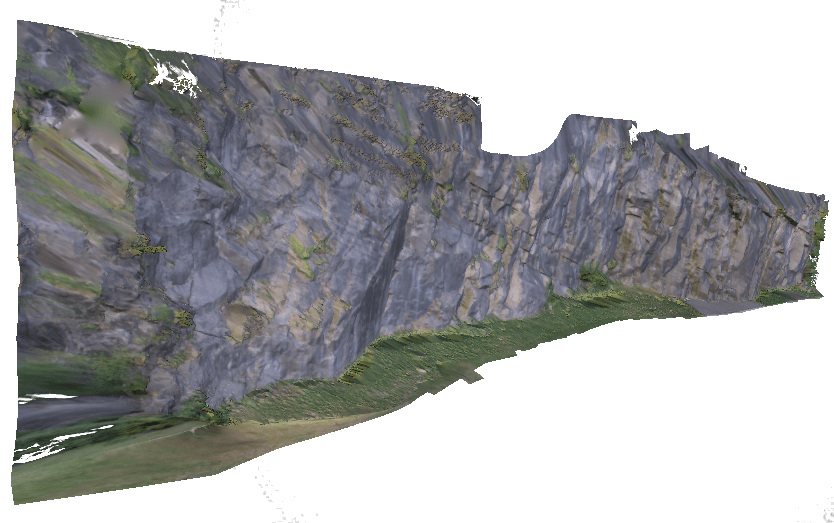
\includegraphics[width=\textwidth]{AvonGorge/Pass1}
        \caption{The model produced using only the first pass of photos at the
        zenithal angle.}
        \label{img:avon-gorge/pass-1}
    \end{subfigure}
    \begin{subfigure}[b]{0.45\textwidth}
        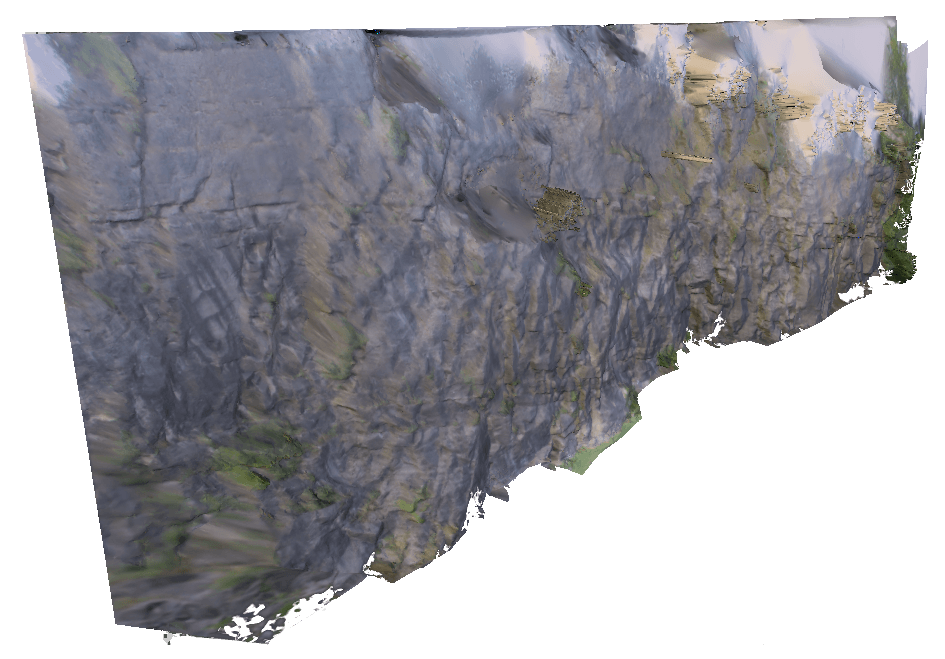
\includegraphics[width=\textwidth]{AvonGorge/Pass2}
        \caption{The model produced using only the second pass of photos at the
        oblique angle.}
        \label{img:avon-gorge/pass-2}
    \end{subfigure}
    \begin{subfigure}[b]{0.9\textwidth}
        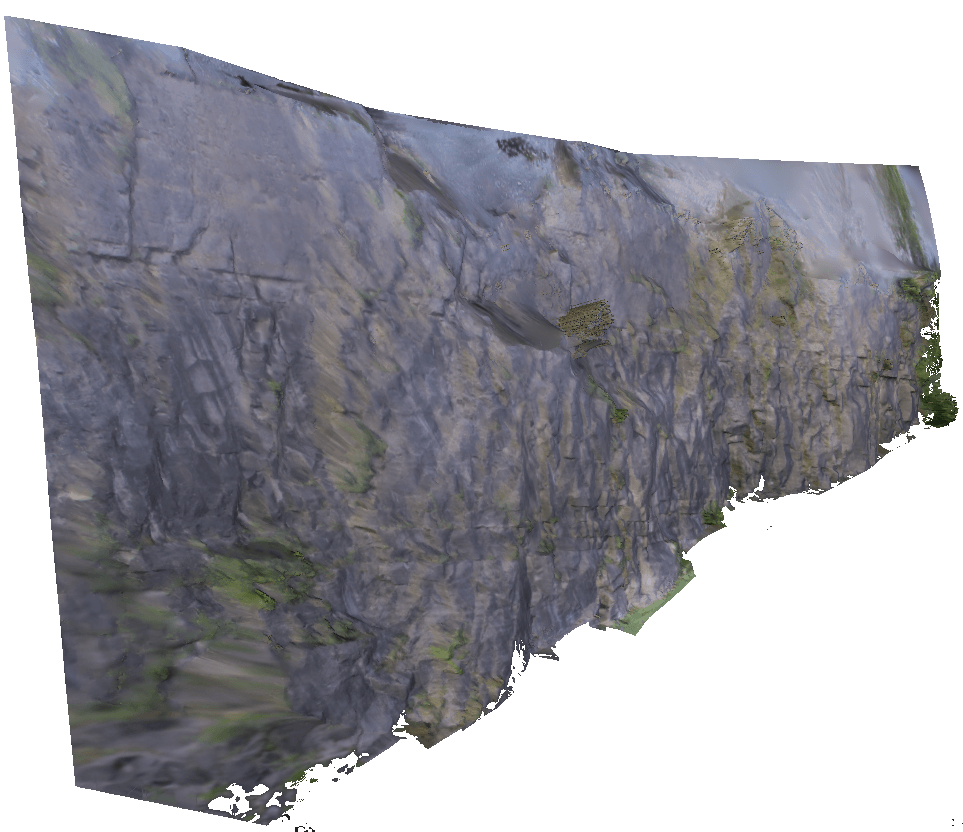
\includegraphics[width=\textwidth]{AvonGorge/Pass2Masked}
        \caption{The model produced using only the second pass of photos,
        masking out the sky.}
        \label{img:avon-gorge/pass-2/masked}
    \end{subfigure}
    \caption{A visual comparison of the relative error induced in the models
    produced in the first and second passes, at zenithal and oblique angles
    respectively.}
    \label{img:avon-gorge/passes}
\end{figure}

\subsubsection{Without GCPs}

\begin{figure}
    \centering
    \begin{subfigure}[b]{0.24\textwidth}
        \includegraphics[width=\textwidth]{AvonGorge/NoGCPs/Orthophoto}
        \caption{The generated orthophoto for the Avon Gorge data set, no 14
        GCPs input.}
        \label{img:avon-gorge/no-gcps/orthophoto}
    \end{subfigure}
    \begin{subfigure}[b]{0.24\textwidth}
        \includegraphics[width=\textwidth]{AvonGorge/NoGCPs/DEM}
        \caption{The generated DEM for the Avon Gorge data set, no 14 GCPs
        input.}
        \label{img:avon-gorge/no-gcps/dem}
    \end{subfigure}
    \begin{subfigure}[b]{0.24\textwidth}
        \includegraphics[width=\textwidth]{AvonGorge/NoGCPs/Overlap}
        \caption{The calculated photographic overlap achieved in the Avon Gorge
        photo dataset no 14 GCPs.}
        \label{img:avon-gorge/no-gcps/overlap}
    \end{subfigure}
    \begin{subfigure}[b]{0.24\textwidth}
        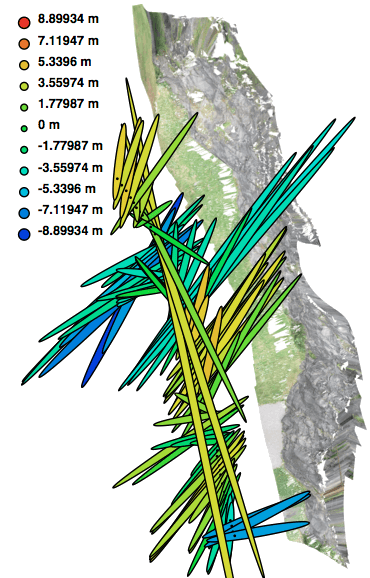
\includegraphics[width=\textwidth]{AvonGorge/NoGCPs/Cameras}
        \caption{The calculated positions of the cameras, along with the errors
        involved in these calculations, representation as ellipses.}
        \label{img:avon-gorge/no-gcps/cameras}
    \end{subfigure}
    \caption{The data produced by PhotoScan from the Avon Gorge horizontal
    imagery, no 14 GCPs input.}
    \label{img:avon-gorge/no-gcps}
\end{figure}

\textbf{Todo: Mention a slope again, and possible cause}
\textbf{Todo: Mention accuracy}
\textbf{Todo: Talk about inaccuracy in camera placement, and how this shows how
useful GCPs are}

\subsubsection{With GCPs}

\begin{figure}
    \centering
    \begin{subfigure}[b]{0.45\textwidth}
        \includegraphics[width=\textwidth]{AvonGorge/WithGCPs/Orthophoto}
        \caption{The generated orthophoto for the Avon Gorge data set, with 14
        GCPs input.}
        \label{img:avon-gorge/with-gcps/orthophoto}
    \end{subfigure}
    \begin{subfigure}[b]{0.45\textwidth}
        \includegraphics[width=\textwidth]{AvonGorge/WithGCPs/DEM}
        \caption{The generated DEM for the Avon Gorge data set, with 14 GCPs
        input.}
        \label{img:avon-gorge/with-gcps/dem}
    \end{subfigure}
    \begin{subfigure}[b]{0.45\textwidth}
        \includegraphics[width=\textwidth]{AvonGorge/WithGCPs/Overlap}
        \caption{The calculated photographic overlap achieved in the Avon Gorge
        photo dataset with 14 GCPs.}
        \label{img:avon-gorge/with-gcps/overlap}
    \end{subfigure}
    \begin{subfigure}[b]{0.45\textwidth}
        \includegraphics[width=\textwidth]{AvonGorge/WithGCPs/GCPs}
        \caption{The positions of the input GCPs.}
        \label{img:avon-gorge/with-gcps/gcps}
    \end{subfigure}
    \caption{The data produced by PhotoScan from the Avon Gorge horizontal
    imagery, with 14 GCPs input.}
    \label{img:avon-gorge/with-gcps}
\end{figure}

\textbf{Todo: Show how slope has resolved itself with GCPs}
\textbf{Todo: Compare accuracy to no GCPs and to Long Ashton}
